\documentclass{standalone}
\usepackage{tikz}
\usetikzlibrary{patterns, positioning}
\usepackage[sfdefault]{ClearSans} %% option 'sfdefault' activates Clear Sans as the default text font
\usepackage[T1]{fontenc}

\begin{document}
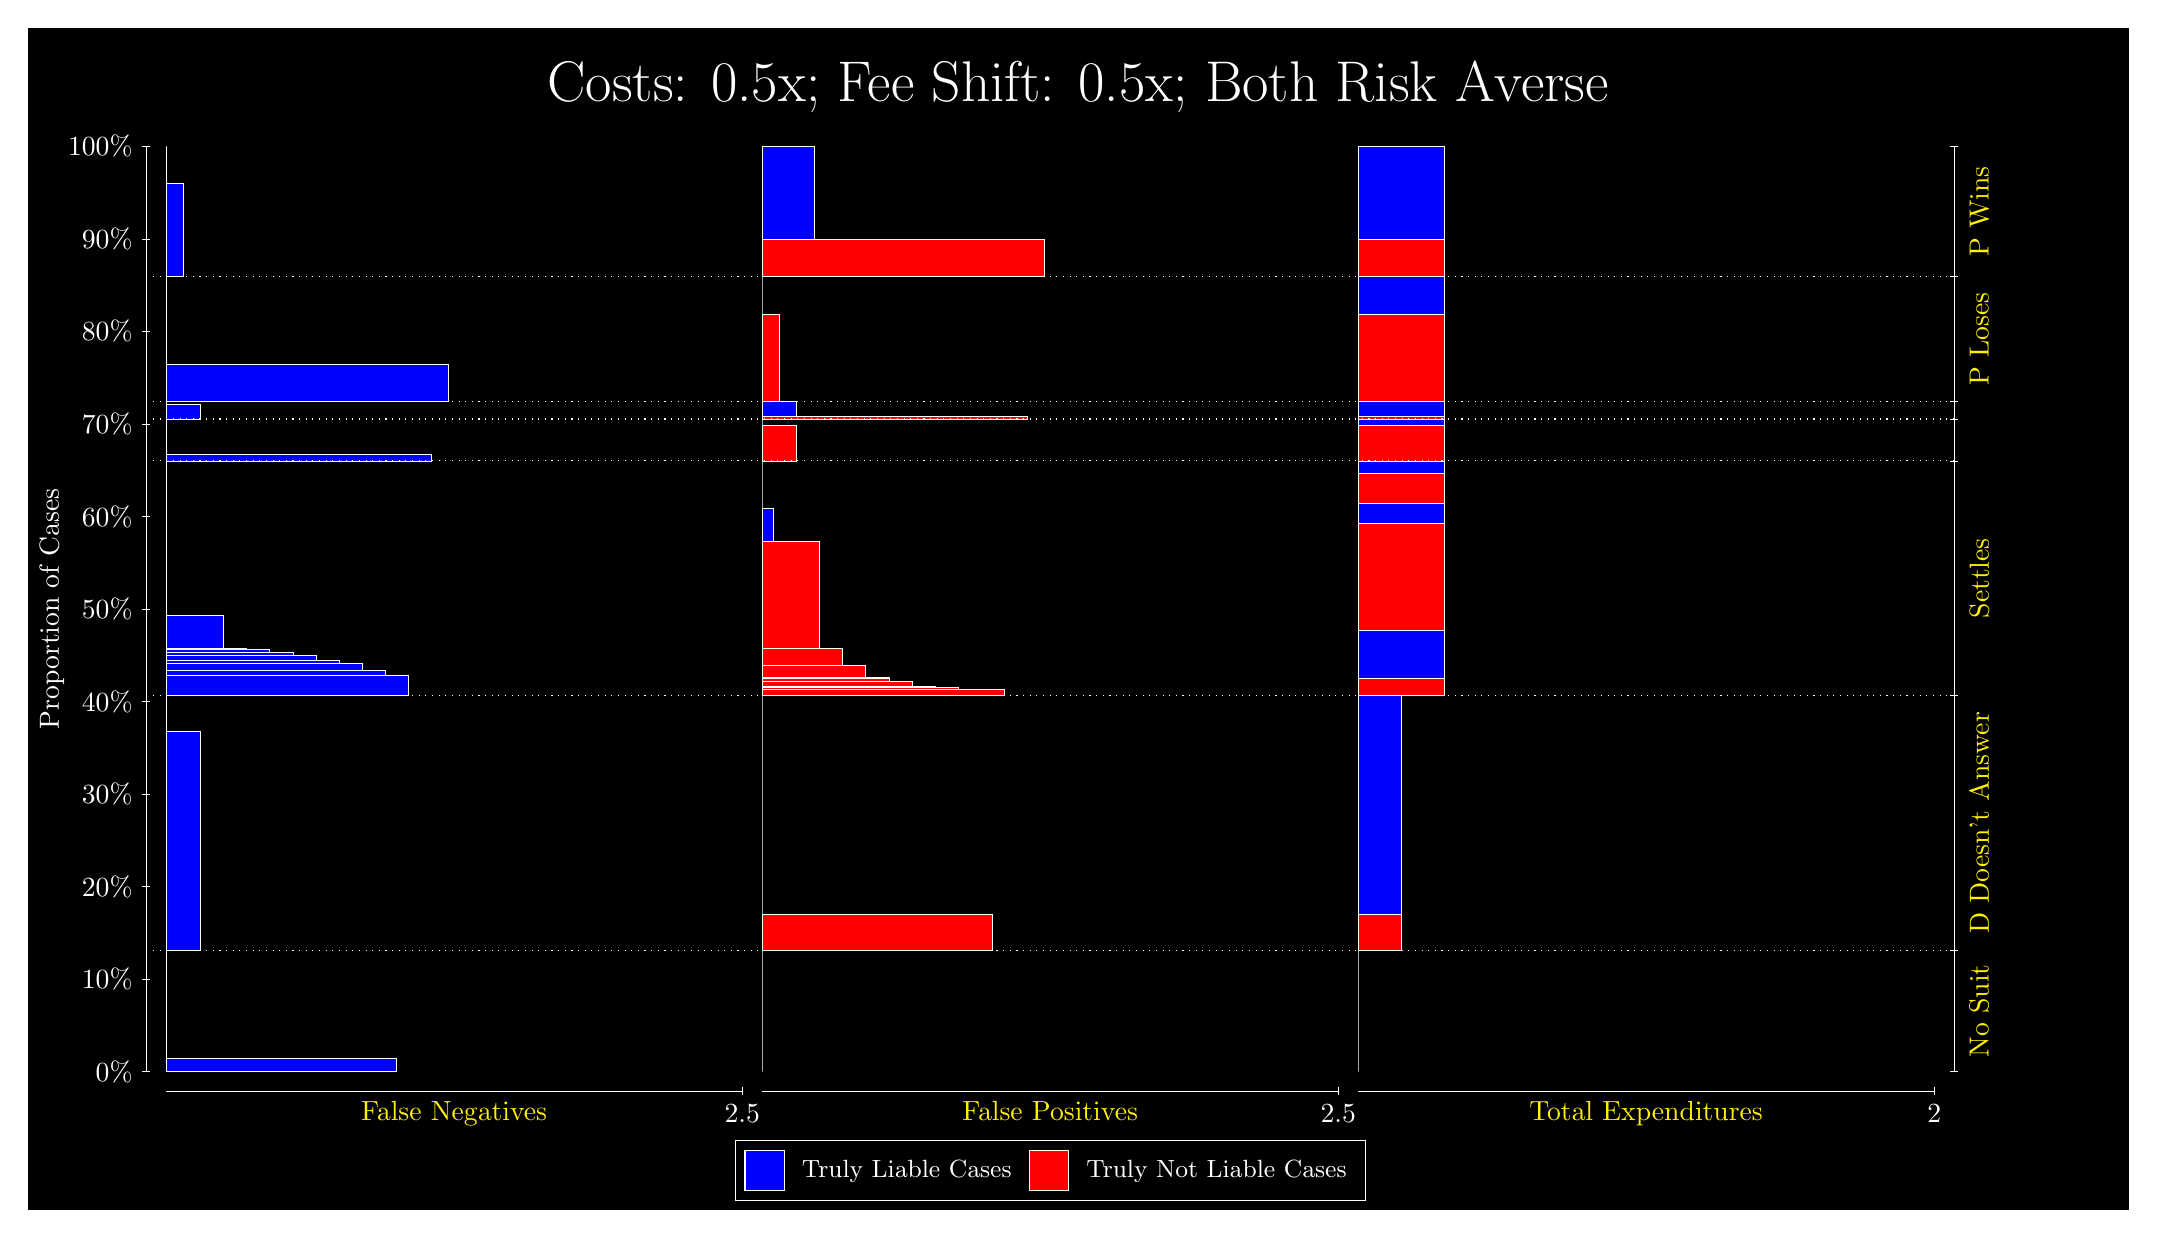
\begin{tikzpicture}
\draw[fill=black] (0,0) rectangle (26.667,15);
\draw[text=white] (0,13.5) rectangle (26.667,15) node[midway] {\huge Costs: 0.5x; Fee Shift: 0.5x; Both Risk Averse};
\draw[white, very thin] (1.5,1.75) -- (1.5,13.5);
\node[rotate=90, text=white, anchor=center] at (0.3, 7.625) {Proportion of Cases};
\draw[white, very thin] (1.45,1.75) -- (1.55,1.75);
\node[text=white, anchor=east] at (1.45, 1.75) {0\%};
\draw[white, very thin] (1.45,2.925) -- (1.55,2.925);
\node[text=white, anchor=east] at (1.45, 2.925) {10\%};
\draw[white, very thin] (1.45,4.1) -- (1.55,4.1);
\node[text=white, anchor=east] at (1.45, 4.1) {20\%};
\draw[white, very thin] (1.45,5.275) -- (1.55,5.275);
\node[text=white, anchor=east] at (1.45, 5.275) {30\%};
\draw[white, very thin] (1.45,6.45) -- (1.55,6.45);
\node[text=white, anchor=east] at (1.45, 6.45) {40\%};
\draw[white, very thin] (1.45,7.625) -- (1.55,7.625);
\node[text=white, anchor=east] at (1.45, 7.625) {50\%};
\draw[white, very thin] (1.45,8.8) -- (1.55,8.8);
\node[text=white, anchor=east] at (1.45, 8.8) {60\%};
\draw[white, very thin] (1.45,9.975) -- (1.55,9.975);
\node[text=white, anchor=east] at (1.45, 9.975) {70\%};
\draw[white, very thin] (1.45,11.15) -- (1.55,11.15);
\node[text=white, anchor=east] at (1.45, 11.15) {80\%};
\draw[white, very thin] (1.45,12.325) -- (1.55,12.325);
\node[text=white, anchor=east] at (1.45, 12.325) {90\%};
\draw[white, very thin] (1.45,13.5) -- (1.55,13.5);
\node[text=white, anchor=east] at (1.45, 13.5) {100\%};

\draw[white, very thin] (24.457,1.75) -- (24.457,13.5);
\draw[white, very thin] (24.407,1.75) -- (24.507,1.75);
\node[anchor=west] at (24.407, 1.75) {};
\draw[white, very thin] (24.407,3.2925) -- (24.507,3.2925);
\node[anchor=west] at (24.407, 3.2925) {};
\draw[white, very thin] (24.407,6.5234) -- (24.507,6.5234);
\node[anchor=west] at (24.407, 6.5234) {};
\draw[white, very thin] (24.407,9.5055) -- (24.507,9.5055);
\node[anchor=west] at (24.407, 9.5055) {};
\draw[white, very thin] (24.407,10.037) -- (24.507,10.037);
\node[anchor=west] at (24.407, 10.037) {};
\draw[white, very thin] (24.407,10.256) -- (24.507,10.256);
\node[anchor=west] at (24.407, 10.256) {};
\draw[white, very thin] (24.407,11.845) -- (24.507,11.845);
\node[anchor=west] at (24.407, 11.845) {};
\draw[white, very thin] (24.407,13.5) -- (24.507,13.5);
\node[anchor=west] at (24.407, 13.5) {};

\draw[white, very thin, fill=blue] (1.75,1.75) rectangle (4.6775,1.9123);
\draw[white, very thin, fill=red] (1.75,1.9123) rectangle (1.75,3.2925);
\draw[white, very thin, fill=blue] (1.75,3.2925) rectangle (2.1891,6.0673);
\draw[white, very thin, fill=red] (1.75,6.0673) rectangle (1.75,6.5234);
\draw[white, very thin, fill=blue] (1.75,6.5234) rectangle (4.8239,6.7783);
\draw[white, very thin, fill=blue] (1.75,6.7783) rectangle (4.5312,6.8444);
\draw[white, very thin, fill=blue] (1.75,6.8444) rectangle (4.2384,6.9307);
\draw[white, very thin, fill=blue] (1.75,6.9307) rectangle (3.9457,6.9715);
\draw[white, very thin, fill=blue] (1.75,6.9715) rectangle (3.6529,7.0365);
\draw[white, very thin, fill=blue] (1.75,7.0365) rectangle (3.3602,7.0767);
\draw[white, very thin, fill=blue] (1.75,7.0767) rectangle (3.0674,7.1098);
\draw[white, very thin, fill=blue] (1.75,7.1098) rectangle (2.7746,7.131);
\draw[white, very thin, fill=blue] (1.75,7.131) rectangle (2.4819,7.5446);
\draw[white, very thin, fill=red] (1.75,7.5446) rectangle (1.75,9.5055);
\draw[white, very thin, fill=blue] (1.75,9.5055) rectangle (5.1167,9.5849);
\draw[white, very thin, fill=red] (1.75,9.5849) rectangle (1.75,10.037);
\draw[white, very thin, fill=blue] (1.75,10.037) rectangle (2.1891,10.219);
\draw[white, very thin, fill=red] (1.75,10.219) rectangle (1.75,10.256);
\draw[white, very thin, fill=blue] (1.75,10.256) rectangle (5.3362,10.73);
\draw[white, very thin, fill=red] (1.75,10.73) rectangle (1.75,11.845);
\draw[white, very thin, fill=blue] (1.75,11.845) rectangle (1.9696,13.026);
\draw[white, very thin, fill=red] (1.75,13.026) rectangle (1.75,13.5);
\draw[white, very thin, fill=red] (9.3189,1.75) rectangle (9.3189,3.1302);
\draw[white, very thin, fill=blue] (9.3189,3.1302) rectangle (9.3189,3.2925);
\draw[white, very thin, fill=red] (9.3189,3.2925) rectangle (12.246,3.7485);
\draw[white, very thin, fill=blue] (9.3189,3.7485) rectangle (9.3189,6.5234);
\draw[white, very thin, fill=red] (9.3189,6.5234) rectangle (12.393,6.599);
\draw[white, very thin, fill=red] (9.3189,6.599) rectangle (12.1,6.6098);
\draw[white, very thin, fill=red] (9.3189,6.6098) rectangle (11.807,6.6264);
\draw[white, very thin, fill=red] (9.3189,6.6264) rectangle (11.515,6.6472);
\draw[white, very thin, fill=red] (9.3189,6.6472) rectangle (11.222,6.7089);
\draw[white, very thin, fill=red] (9.3189,6.7089) rectangle (10.929,6.7437);
\draw[white, very thin, fill=red] (9.3189,6.7437) rectangle (10.929,6.7521);
\draw[white, very thin, fill=red] (9.3189,6.7521) rectangle (10.636,6.9104);
\draw[white, very thin, fill=red] (9.3189,6.9104) rectangle (10.344,7.1208);
\draw[white, very thin, fill=red] (9.3189,7.1208) rectangle (10.051,8.4843);
\draw[white, very thin, fill=blue] (9.3189,8.4843) rectangle (9.4652,8.8978);
\draw[white, very thin, fill=blue] (9.3189,8.8978) rectangle (9.3189,9.5055);
\draw[white, very thin, fill=red] (9.3189,9.5055) rectangle (9.758,9.9572);
\draw[white, very thin, fill=blue] (9.3189,9.9572) rectangle (9.3189,10.037);
\draw[white, very thin, fill=red] (9.3189,10.037) rectangle (12.686,10.074);
\draw[white, very thin, fill=blue] (9.3189,10.074) rectangle (9.758,10.256);
\draw[white, very thin, fill=red] (9.3189,10.256) rectangle (9.5384,11.371);
\draw[white, very thin, fill=blue] (9.3189,11.371) rectangle (9.3189,11.845);
\draw[white, very thin, fill=red] (9.3189,11.845) rectangle (12.905,12.318);
\draw[white, very thin, fill=blue] (9.3189,12.318) rectangle (9.9776,13.5);
\draw[white, very thin, fill=red] (16.888,1.75) rectangle (16.888,3.1302);
\draw[white, very thin, fill=blue] (16.888,3.1302) rectangle (16.888,3.2925);
\draw[white, very thin, fill=red] (16.888,3.2925) rectangle (17.437,3.7485);
\draw[white, very thin, fill=blue] (16.888,3.7485) rectangle (17.437,6.5234);
\draw[white, very thin, fill=red] (16.888,6.5234) rectangle (17.986,6.7437);
\draw[white, very thin, fill=blue] (16.888,6.7437) rectangle (17.986,7.3495);
\draw[white, very thin, fill=red] (16.888,7.3495) rectangle (17.986,8.713);
\draw[white, very thin, fill=blue] (16.888,8.713) rectangle (17.986,8.9679);
\draw[white, very thin, fill=red] (16.888,8.9679) rectangle (17.986,9.3449);
\draw[white, very thin, fill=blue] (16.888,9.3449) rectangle (17.986,9.5055);
\draw[white, very thin, fill=red] (16.888,9.5055) rectangle (17.986,9.9572);
\draw[white, very thin, fill=blue] (16.888,9.9572) rectangle (17.986,10.037);
\draw[white, very thin, fill=red] (16.888,10.037) rectangle (17.986,10.074);
\draw[white, very thin, fill=blue] (16.888,10.074) rectangle (17.986,10.256);
\draw[white, very thin, fill=red] (16.888,10.256) rectangle (17.986,11.371);
\draw[white, very thin, fill=blue] (16.888,11.371) rectangle (17.986,11.845);
\draw[white, very thin, fill=red] (16.888,11.845) rectangle (17.986,12.318);
\draw[white, very thin, fill=blue] (16.888,12.318) rectangle (17.986,13.5);
\draw[white, dotted] (1.5,3.2925) -- (24.457,3.2925);
\draw[white, dotted] (1.5,6.5234) -- (24.457,6.5234);
\draw[white, dotted] (1.5,9.5055) -- (24.457,9.5055);
\draw[white, dotted] (1.5,10.037) -- (24.457,10.037);
\draw[white, dotted] (1.5,10.256) -- (24.457,10.256);
\draw[white, dotted] (1.5,11.845) -- (24.457,11.845);
\draw[white, very thin] (1.75,1.5) -- (9.0689,1.5);
\node[text=yellow, anchor=north] at (5.4094, 1.5) {False Negatives};
\draw[white, very thin] (9.0689,1.45) -- (9.0689,1.55);
\node[text=white, anchor=north] at (9.0689, 1.45) {2.5};

\draw[white, very thin] (9.3189,1.5) -- (16.638,1.5);
\node[text=yellow, anchor=north] at (12.978, 1.5) {False Positives};
\draw[white, very thin] (16.638,1.45) -- (16.638,1.55);
\node[text=white, anchor=north] at (16.638, 1.45) {2.5};

\draw[white, very thin] (16.888,1.5) -- (24.207,1.5);
\node[text=yellow, anchor=north] at (20.547, 1.5) {Total Expenditures};
\draw[white, very thin] (24.207,1.45) -- (24.207,1.55);
\node[text=white, anchor=north] at (24.207, 1.45) {2};

\node[text=yellow, centered, rotate=90] at (24.777, 2.5212) {No Suit};
\node[text=yellow, centered, rotate=90] at (24.777, 4.9079) {D Doesn't Answer};
\node[text=yellow, centered, rotate=90] at (24.777, 8.0144) {Settles};


\node[text=yellow, centered, rotate=90] at (24.777, 11.05) {P Loses};
\node[text=yellow, centered, rotate=90] at (24.777, 12.672) {P Wins};

\draw (12.978300999999998,1.5) node[draw=none] (baseCoordinate) {};
\begin{scope}[align=center]
        \matrix[scale=0.5, draw=white, below=0.5cm of baseCoordinate, nodes={draw}, column sep=0.1cm]{
            \node[rectangle, draw, minimum width=0.5cm, minimum height=0.5cm, fill=blue] {}; &
            \node[draw=none, font=\small, text=white] (B) {Truly Liable Cases}; &
            \node[rectangle, draw, minimum width=0.5cm, minimum height=0.5cm, fill=red] {}; &
            \node[draw=none, font=\small, text=white] (B) {Truly Not Liable Cases}; \\
            };
\end{scope}

\end{tikzpicture}
\end{document}